%
% File document.tex
%
% Contact: gdzhou@suda.edu.cn
%%
%% Based on the style files for ACL2008 by Joakim Nivre and Noah Smith
%% and that of ACL2010 by Jing-Shin Chang and Philipp Koehn


\documentclass[11pt]{article}
\usepackage{acl-hlt2011}
\usepackage{times}
\usepackage{latexsym}
\usepackage{amsmath}
\usepackage{multirow}
\usepackage{url}
\usepackage{graphicx}
\DeclareMathOperator*{\argmax}{arg\,max}
\setlength\titlebox{6.5cm}    % Expanding the titlebox

\title{Language detection in tweets}

\author{Siddharth Subramanian \\
  University of Texas at Austin\\
  {\tt sid@cs.utexas.edu} \\}

\date{}

\begin{document}
\maketitle
\begin{abstract}
This paper describes an approach to tackle the problem of language detection in tweets. Analysis of Twitter data can be difficult because of the constraint on the length of tweets, and also because of multi-lingual posts. Knowledge about the language of a tweet can help greatly in processing the data better -- especially in tasks like Twitter sentiment analysis. An important task in training machine learning algorithms for this task is to get labeled data. This paper describes an approach to automatically label twitter data in an unsupervised manner. The labeled data obtained by this unsupervised labeling algorithm is then used to create a language model, which is utilized to detect languages in tweets. The technique presented in this paper gives promising results, and can be easily extended to other languages with minimum effort. Further extensions to the labeling approach using geo-located tweets are suggested; training our model using tweets collected from ``reliable'' regions that have a high proportion of speakers of a language further increases the accuracy of language detection.
\end{abstract}

\section{Introduction}
Twitter is a microblogging site which allows users to post short messages (which are no more than 140 characters long). Since this service is very popular, performing sentiment analysis over twitter posts is a cost-effective way of understanding the opinion of general public about a particular issue or product. Sentiment analysis involves a lot of text processing and training data. However, one of the main reasons for low accuracy in sentiment analysis is that the posts are multi-lingual, and the system is trained usually using only one language. This is where language detection in twitter posts becomes important.

Language identification in text is not a new problem, though. The usual character n-gram approach trained on huge amounts of text gives accurate results in most cases. This approach does not work well on twitter data because of two main reasons: (1) the posts are very small and we do not have enough character n-grams from the post to characterize the language, (2) because of constraints on length of tweets, users create new words (for example, {\em smthng} for ``something'') which results in an entirely new style when compared to the formal text used for training data (like EuroParl).

Obtaining labeled data from twitter is a laborious task. Even though there is a {\em lang} field in Twitter API's \footnote[1]{https://dev.twitter.com/docs/api/1/get/search} metadata, it is often inaccurate and is not a reliable method for identifying the language of twitter posts. One way to obtain large amounts of labeled data is to find the proportion of valid word types of a particular language $L$ in the tweet, and to assign that label $L$ if the proportion is significantly high. This forms the basis of unsupervised labeling algorithm, which is explained in subsequent sections.

\section{Related work}
A lot of work has been done in analyzing the language of tweets. 
Hong et al. (2011) conducted a few experiments on a very large number of tweets (62 million), which were aimed at characterizing Twitter data. It was found that only around 50\% of the tweets are in English, showing that training models only in English would not be effective for analyzing Twitter data.
A study conducted by Semiocast (2010) reveals that English, Japanese, Portuguese, Malay and Spanish are the top 5 most used languages in Twitter, and that English constitutes only half of the tweets from around the world. 

In Han and Baldwin (2011), a method to identify and normalize out-of-vocabulary words is described. An ill-formed word is first detected using dependency features of the Stanford parser (Klein and Manning, 2003; de Marneffe et al., 2006). A set of suggestions are generated, and features like lexical edit distance, phonemic edit distance, and longest common subsequence are used to select the most appropriate candidate. However, the study is limited to the English language only.
The work by Tromp and Pechenizkiy (2011) studies the problem of language identification on short text like tweets. A graph-based approach which considers character trigrams as well as the order of words is suggested to identify the language.

Ceylan and Kim (2009) deals with the problem of language identification of search engine queries, which is similar to our research because both these problems deal with small text inputs. It is pointed out in their work that the word n-gram approach, with $n > 1$ would not help in language identification of search queries. A decision tree classifier is built by using 3 features: character n-gram, word-based approach, and morphological feature (prefix and suffix), for detecting the language of the query. It is also shown that when the classifier included geographical information of the users, the performance received a boost. This could be useful information in our problem as well, because there are a lot of geo-tagged tweets which contain information about the location of users, and would be interesting to see the impact on the accuracy of language detection in twitter domain.

Carter et al (2012) used labeled data and other twitter parameters for language detection. But this method relies on a lot of factors other than the text in tweets, and may be time-consuming. One of the contributions of this paper is that, a labeled dataset used for this research is published on the web, which is useful for further research on Twitter analysis. This work improves the language detection by considering other factors like blogger's previous tweets (blogger prior), the conversation in which the tweet occurs (converstation prior), tags used in the tweets (tag prior) and URLs mentioned in the tweets (link prior). Even before analyzing the actual text in the unlabeled tweet, a prior probability distribution is estimated by using these factors. This is then combined with the language detected for the actual tweet to give the final prediction. Some important results of this research work are: (1) accuracy of language detection increases when the system is trained on tweets rather than formal text, (2) exploiting the priors mentioned above gives significant improvement in the accuracy of language prediction of a tweet.

The research by Chen (2011) \footnote[2]{http://blog.echen.me/2011/05/01/unsupervised-language-detection-algorithms} employs unsupervised method for filtering non-English tweets. In this method, Expectation-Maximization algorithm is run on tweets to create two clusters -- English, and non-English tweets. This approach relies heavily on the text contained in the tweets.

In this paper, we suggest ways for using unsupervised methods to avoid the task of manually labeling a huge amount of tweets. A similar problem was also tackled by Nigam et al. (2000) in which they suggest a combination of Naive Bayes and EM to classify text. Using this method, we need very little labeled data in order to classify large amounts of unlabeled text. Our method does not need any labeled text and is based on wordlists of languages and a simple heuristic. It relies on the fact that huge amounts of text would eventually help in converging to the correct model, with negligible errors. There are abundant tweets available via the Twitter API, and hence this method works very well.

\section{High-confidence dictionary-based labeling algorithm for collecting training data}
As mentioned earlier, getting labeled twitter data is not a trivial task. All methods which were based on training data used manually labeled tweets for their learning algorithms. However, this might restrict the number of tweets used for training to a few thousands. The language identification algorithm could perform better if it is trained using a lot more tweets. For this, an unsupervised way of getting labeled data is proposed. The method is quite simple -- use words from dictionary of languages and count the number of valid words and the proportion of such valid words from each language that has appeared in a tweet. If these values for a language $L$ in the tweet exceeds a certain threshold, then it can be labeled with $L$. We used Wiktionary, which is a freely available source of wordlists, for building wordlists for languages. Initial experiments showed that the unsupervised labeling algorithm achieves more than 89\% accuracy when the threshold for the number of valid words is set to 4 and proportion of valid words was set to 0.6. If the criterion is not met, the tweet is ignored. In this way, a lot of accurately labeled tweets can be collected. Even though all tweets might not be labeled, the fact that the labeling operation is unsupervised gives a powerful method to acquire large amounts of labeled training data. Also, slight inaccuracies in identifying the labels using this approach are negligible, as the number of tweets is very high.

The above method was run on a dataset containing more than 10 million tweets, and the number of tweets that were labeled by the above algorithm is tabulated in Table 1.

\begin{table}
\begin{center}
\small
\begin{tabular}{|c|c|}
\hline
\textbf{Language} & \textbf{Number of tweets labeled} \\
\hline
English & 1157034 \\
Spanish & 772014 \\
German & 20548 \\
French & 48766 \\
Dutch & 142666 \\ \hline
\end{tabular}
\caption{\footnotesize Number of tweets used for obtaining language models}
\end{center}
\end{table}

The first step is to acquire labeled tweets using the technique described above. Also, currently, the languages that would be considered are -- English, Spanish, German, French, Dutch and Unknown. If enough words are not found from these languages in a tweet, it is ignored. A tweet is labeled `Unknown' if the number of words in the tweet that does not match any of the known dictionary words exceeds a certain threshold. For example, if a tweet contains 10 words, out of which only 1 word is recognizable as English, then it means that the tweet contains 90\% unknown words and hence labeled `Unknown'.	

Once a set of labeled tweets is obtained, a language model is built for each language using this training data. Each language's model is a set of character n-grams sorted in descending order of frequncy of their occurrence. Only the top 500 such n-grams are retained. Now, for a given input tweet $T$, its language is detected by using rank-correlation as shown below.\\

$ score(l) = \sum_{n \in ngrams(T)} | r_{model}(n) - r_T(n) | $
\\
\par
$ label(T) = \operatorname*{arg\,min}_{l \in \{S\}} score(l) $ \\

\par
where,
\begin{itemize}
\item $l$ = language
\item $S$ is the set of supported languages
\item $S$ is the set of supported languages
\item $score(l)$ = the rank correlation score assigned to language $l$
\item $label(T)$ = the final label predicted by the model for tweet $T$
\item $r_{model}(n)$ = Rank of the n-gram $n$ in the list of n-grams for the language $l$
\item $r_T(n)$ = Rank of n-gram $n$ in the list of n-grams generated from the tweet $T$
\end{itemize}

In other words, the \emph{distance} between the given tweet and a language $l$ is calculated based on the ranks of character n-grams. Then, the language which is at the least distance from the given tweet is the predicted label of our model.
Even though there have been approaches based on character n-grams, our approach is different in the sense that -- the data is obtained automatically from twitter, and a huge amount of tweets will be used for generating the language models, without using formal text from any other sources. We expect this to be a better representative of the actual tweets, and hence produce better results.

The High-confidence Dictionary-based labeling algorithm (HCDL) is used only to get labeled training data, and not for the actual prediction task. For the language identification task, TextCat is used on our model described above. This is explained in the next section.

\section{Language detection}
For classifying an unlabeled tweet, the character n-grams of the tweet were generated (where n ranges from 1 to 5), and the correct language was identified using TextCat, a text categorization tool. In order to generate a model that is compatible with TextCat, the n-grams were sorted in descending order of their counts. Also, not all the n-grams were included in the language model. Top 500 character n-grams were taken into consideration because there is a possibility of error as the counts of n-grams decreases. Initial experiments show that top 500 n-grams give best results (Figure 2).

TextCat performs language detection by generating n-grams of the input text and comparing it with the language models on which it has been trained. For our experiments we used the models that we obtained using our unsupervised labeling method. TextCat assigns a {\em distance} or {\em score} for each language, and the predicted language is the one corresponding to the least distance from the language model.

In order to identify languages more accurately, the {\em blogger prior} was also calculated for the author of each tweet as in Carter et al. (2012). This was done by obtaining the last few tweets (around 150-200) of an author, and calculating the scores for each of the five languages. This language prediction task of the tweets of bloggers was also done using TextCat trained on our models. Let $T$ = \{ $t_1, t_2, ..., t_k$\} be the previous $k$ tweets of a user/blogger. The blogger profile is calculated as follows : for each tweet $t_i \in T$, find the scores calculated by TextCat for each language $L$. The blogger profile is then the vector ($s_1, s_2, ..., s_l$) where $l$ is the number of languages over which TextCat is trained, and $s_i$ is the average score calculated by TextCat for language $i$ over all the $k$ tweets.
Once the blogger prior is calculated, it is combined with the prediction for actual tweet using a weight factor $w$ as follows: \\
\begin{eqnarray}
{\lambda}_{combined} = w * {\lambda}_{blogger} + (1 - w) * {\lambda}_{tweet} 
\end{eqnarray}
where $w$ is the weightage given to our prior knowledge about the blogger, ${\lambda}_{blogger}$ is the score calculated by TextCat on the blogger's tweets, ${\lambda}_{tweet}$ is the score calculated by TextCat on the given input tweet.

As mentioned in Carter et al. (2012), including the blogger prior does improve the accuracy of language prediction task. It was seen that with this single additional prior, overall accuracy of over 96\% was achieved by our language models. More details are discussed in the results section.

\section{Data set}
This section describes the dataset that was used for carrying out the experiments. Carter et al. (2012) have provided a development, training and testing set for the five languages -- English, Spanish, French, Dutch and German. We used their development set for tuning our parameters (such as number and proportion of valid words, the weight factor for combining tweet and blogger profiles). For the results that are reported in this paper, their testing set was used. The breakup of the number of tweets in development, training and testing set in their dataset is given in Table 2. It should be noted that some tweets were not available due to certain reasons (users protected their tweets, or deleted their accounts). Hence the number of tweets that were used in the actual work by Carter et al (2012) is different from what was used in our work.

\begin{table}
\begin{center}
\small
\begin{tabular}{|c|c|}
\hline
\textbf{Dataset} & \textbf{Number of tweets} \\
\hline
Development & 401 \\
Training & 2003 \\
Testing & 1987  \\ \hline
\end{tabular}
\caption{\footnotesize Number of tweets in the dataset provided by Carter et al (2012)}
\end{center}
\end{table}

The number of tweets that were labeled (the ones that were used to build the language model) for each language is tabulated in Table 1.


\section{Results}
In this section, the results of certain experiments are reported. The first step in proposed approach is to identify the language of tweets based on the number (and the proportion) of valid words. Some sample data \footnote[3]{The dataset was taken from the development data used in http://ilps.science.uva.nl/resources/twitterlid} was taken, and this method of labeling was employed on that sample set. The dataset contains 401 tweets, which have been labeled manually with the language. For this experiment, the labels were removed, and the tweets were fed as input to our algorithm.

\begin{figure}[ht]
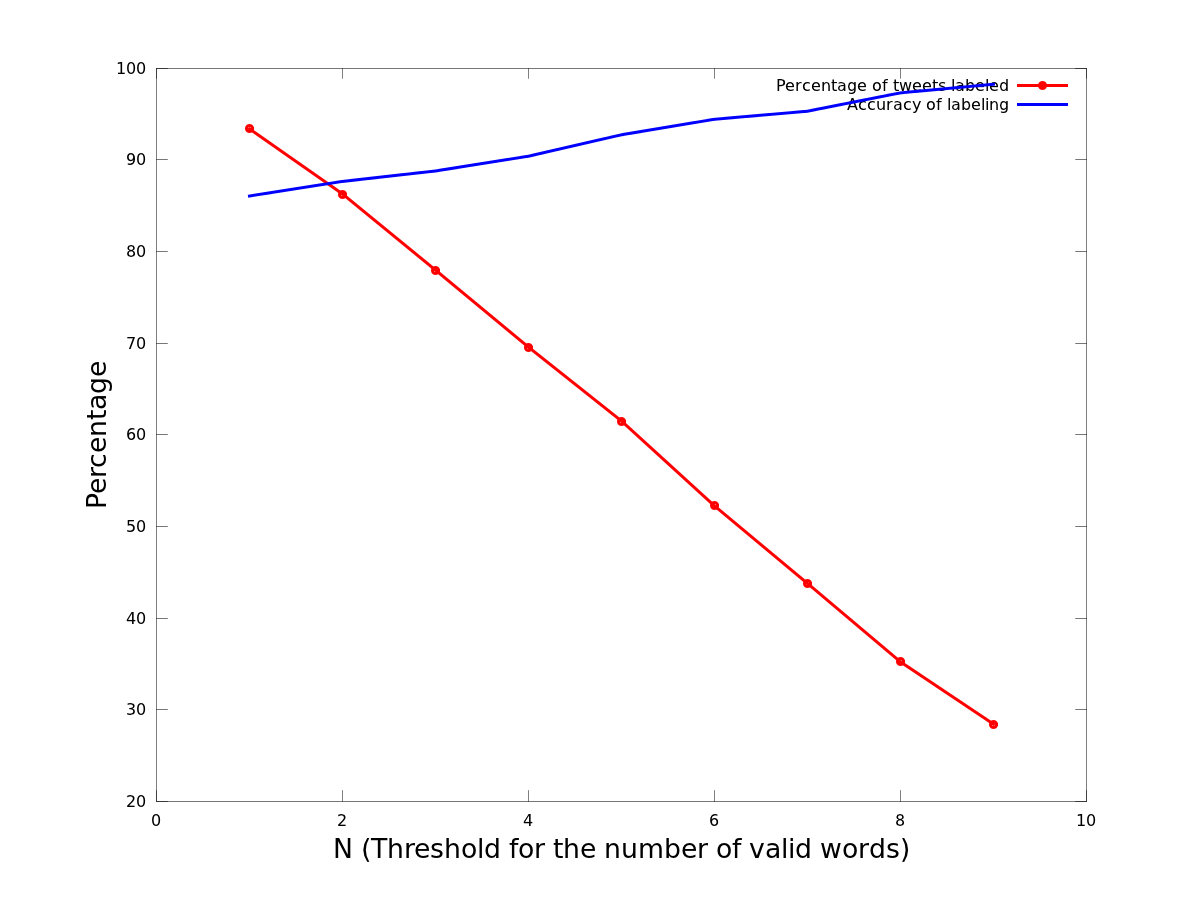
\includegraphics[scale=0.4]{accuracy_words.png}
\caption{\footnotesize Accuracy of labeling method based on number of valid words in a tweet}
\label{fig:s2}
\end{figure}


Figure 1 shows the overall accuracy of the labeling algorithm along with various values for the threshold for minimum number of valid words in a tweet required for classification. It also shows the number of tweets that were actually classified, that is, the number of tweets that were not ignored. As expected, the accuracy of labeling increases as N increases (the smooth line with `X's, in Figure 1). We can observe that at N=4, the accuracy is above 89\%, and that more than 75\% of tweets were labeled. As N increases, the number of labeled tweets falls rapidly (line with squares, in Figure 1). This experiment serves as a proof of concept for the effectiveness of labeling based on number of valid words in a tweet. The results are promising, and a large number of labeled tweets were obtained using this method.

{\textbf {Baseline: }}  In order to measure the effectiveness of our results, the dictionary based approach was used as a baseline method. In this approach, the tweet is labeled with the language from which it has the maximum number of valid words. The set of valid words for each language is obtained from the dictionary of that language. For example, if a tweet contains 3 English words, 1 Spanish word, then that tweet would be classified as an English tweet by this method. This is a fast and simple method to classifiy tweets -- however it is not suitable for Twitter dataset because of the slang and shortened words, which are not found in dictionaries. This is seen clearly from the classification accuracy shown in Table 5. It fails to achieve an overall accuracy of 90\% percent, which has been achieved by the state-of-the-art techniques.

{\textbf {Language prediction without blogger prior: }}  First, the language prediction task was run without taking the blogger prior into consideration. The results are summarized in Table 3.

\begin{table*}
\begin{center}
\small
\begin{tabular}{|c|c|c|c|c|c|c|}
\hline
\textbf{} & \textbf{English} & \textbf {German} & \textbf{Spanish} & \textbf{Dutch} & \textbf{French} & \textbf{Precision} \\
\hline
English    &        380       &       1          &        5         &       2        &        3        &      \textbf{97.19} \\
German     &         17       &     363          &        0         &       6        &        2        &      \textbf{93.56} \\
Spanish    &         19       &       6          &      399         &       5        &        7        &      \textbf{91.53} \\
Dutch      &         23       &       7          &        4         &     320        &        2        &      \textbf{89.88} \\
French     &         28       &       8          &        7         &       3        &      370        &      \textbf{88.94} \\
\hline
\textbf{Recall}&\textbf{81.37}& \textbf{94.29}   & \textbf{96.144}  & \textbf{95.24} & \textbf{96.35}  &      \textbf{} \\
\hline
\multicolumn{7}{|c|}{\textbf{Overall accuracy = 92.2}} \\\hline
\end{tabular}
\caption{\footnotesize Performance of language prediction task based on our model without using blogger prior. The leftmost column represents the actual label, topmost row represents the predicted labels. The numbers denote the number of tweets classified.}
\end{center}
\end{table*}

\begin{table*}
\begin{center}
\small
\begin{tabular}{|c||c|c||c|c||c|c||c|c|}
\hline
\textbf{Language} & \multicolumn{2}{|c||}{\textbf {No geo, no BP}} & \multicolumn{2}{|c||}{\textbf{No geo, with BP}} & \multicolumn{2}{|c||}{\textbf{Geo, no BP}} & \multicolumn{2}{|c|}{\textbf{Geo, BP}} \\
\hline
 & Precision & Recall & Precision & Recall & Precision & Recall & Precision & Recall \\
\hline
English   & 97.19 & 81.37 & 92.68 & 86.36 & 96.93 & 83.85 & 95.12 & 90.69 \\
German    & 93.56 & 94.28 & 89.16 & 91.36 & 92.78 & 94.74 & 98.79 & 98.79 \\
Spanish   & 91.51 & 96.14 & 96.42 & 96.43 & 91.72 & 96.16 & 97.62 & 98.61 \\
French    & 88.94 & 96.35 & 89.29 & 92.59 & 89.18 & 96.61 & 95.23 & 98.53 \\
Dutch     & 89.89 & 95.24 & 94.12 & 95.52 & 91.97 & 93.50 & 98.53 & 98.7 \\
\hline
\textbf{Overall accuracy} & \multicolumn{2}{|c||}{\textbf{92.2}} & \multicolumn{2}{|c||}{\textbf{96.76}} & \multicolumn{2}{|c||}{\textbf{92.702}} & \multicolumn{2}{|c|}{\textbf{97.01}} \\
\hline
\end{tabular}
\caption{\footnotesize Summary of results. In the first row, \emph{BP} = blogger prior, \emph{No geo} indicates the model that was trained on all tweets, \emph{Geo} indicates the model that was trained on ``highly reliable'' regions by taking geo-location into consideration. }
\end{center}
\end{table*}

\begin{table}
\begin{center}
\small
\begin{tabular}{|c|c|}
\hline
\textbf{Approach} & \textbf{Accuracy} \\
\hline
Dictionary based baseline                 & 71.67 \\
Carter et al (2012) with blogger prior    & 97.4 \\
Carter et al (2012) without blogger prior & 92.4 \\
Our model with blogger prior ($w$ = 1)    & 95.76 \\
Our model with tweet text only ($w$ = 0)  & 92.2 \\
Our model with combined prior ($w$ = 0.4) & 97.01 \\

\hline
\end{tabular}
\caption{\footnotesize Comparison with other approaches and baselines}
\end{center}
\end{table}


It can be seen from Table 3 that, the model identifies the correct language with more than 92\% accuracy overall. However, this can still be improved by using the blogger prior.

Another factor that affected the accuracy was the number of n-grams to be considered while generating the language model. TextCat uses these n-grams to detect the languages. We found that the top 500 n-grams were giving best results. This can be attributed to the fact that, as the number of n-grams considered increases, there are more chances of errors as well, since the models were generated based on a heuristic. Figure 2 shows the accuracy as the number of n-grams increases. We can see clearly that the highest accuracy is achieved for the case when we consider the top 500 n-grams.

\begin{figure}[ht]
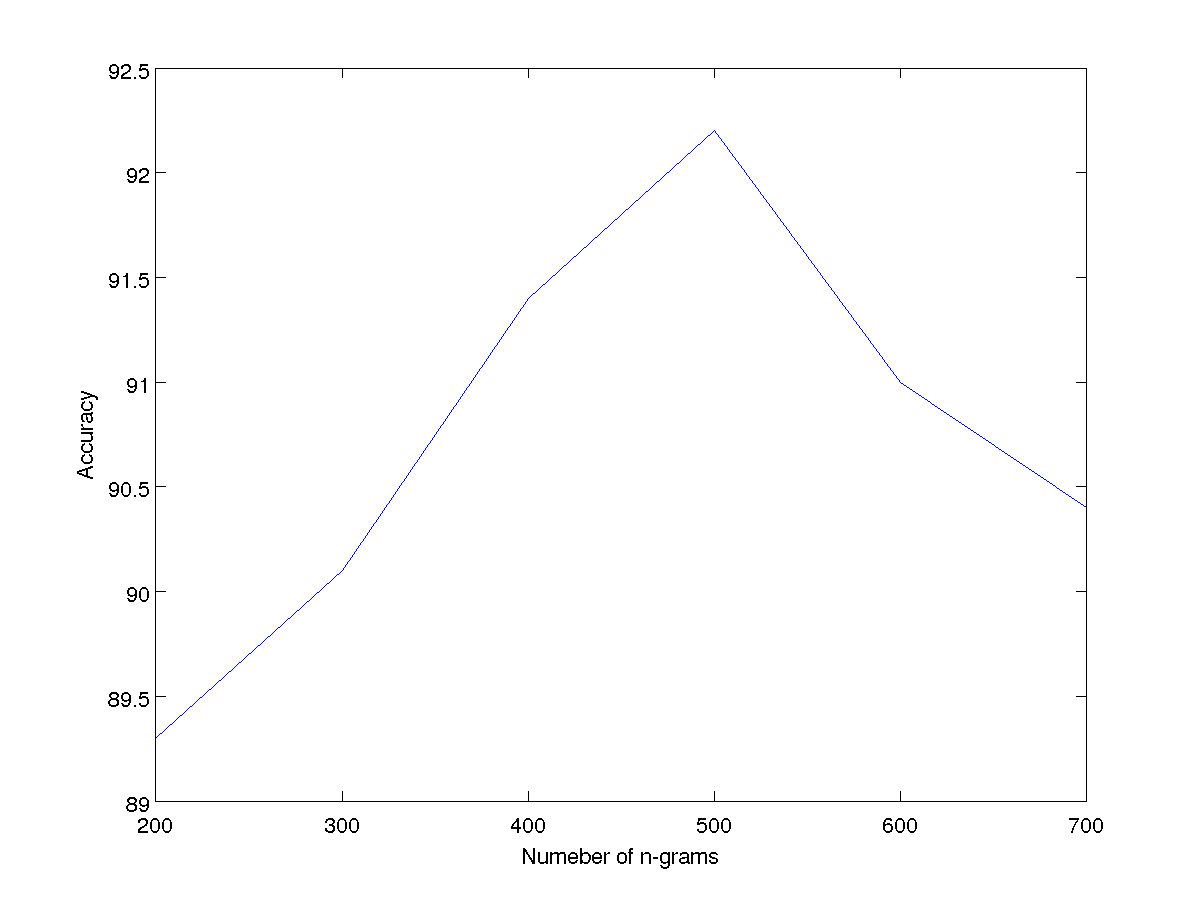
\includegraphics[scale=0.35]{ngramsVsAccuracy.png}
\caption{\footnotesize Accuracy of language detection Vs number of n-grams considered in the model}
\label{fig:s3}
\end{figure}


{\textbf {Language prediction using blogger prior: }} Now we describe the results obtained by including the blogger prior for every tweet that is being classified. Best results were obtained by using $w = 0.4$ in equation (1) for calculating scores for every language. The results of predicting the language using our model with blogger prior is shown in Table 4. It can be seen that the accuracy has improved by around 4\%, and all languages are predicted correctly with an accuracy of at least 95\%.

In order to show that adding blogger prior improves accuracy, we ran the experiment with two simple baselines: (1) Our model with tweet text only ($w$ = 0), and (2) Our model with blogger prior only ($w$ = 1).

The first baseline is equivalent to the case where there was no blogger prior taken into consideration while predicting the languages -- this gave an accuracy of 92.2\%.

In the second baseline, the language for the tweet was predicted as follows: for each input tweet, the author's blogger prior was given full weightage, and the tweet was labeled with the author's language only, without considering the tweet text. For example, if the blogger prior for a tweet posted by a user $U$ indicates that the author is tweeting in English, then all the tweets in the dataset that were written by the user $U$ were labeled as English. As we can see in Table 5, this gave an accuracy of 95.76\%.

However, combining the blogger prior (having $w$ = 0.4) with our prediction on tweet text boosts the accuracy even further, thus adding value to the process of language identification.

\subsection{Tweets in unknown languages}
In our approach, we also introduce an explicit `Unknown' label for those tweets which are not in one of the 5 languages (English, Spanish, French, Dutch, German). Carter et al (2012) had datasets only for these 5 languages because they did not deal with unknown languages. In order to measure the performance of our approach, we created a development and test set containing 500 tweets each, for unknown languages. Tweets were collected from regions like China, Japan, Korea, Saudi Arabia, Malaysia, Singapore etc. and were manually verified to ensure that they were not in any of the 5 languages that we support. On running the prediction task on the unknown tweets, we got an overall accuracy of 91.1\% on the dataset for `Unknown' tweets. To get a better idea of the performance of our model, 100,000 geolocated tweets were collected from the Twitter stream, and our model was used to predict languages of \emph{all} the tweets on this set. Figure 3 shows the plot of the `Unknown' language over the surface of the earth. It can be seen that most unknown tweets are from the regions where the 5 supported languages are not spoken. However, after examining a similar plot for English, we could observe that our approach had labeled a lot of tweets from Indonesia and Malaysia regions as English, which are erroneous. The number of unknown tweets from that region are larger than the number that is actually being shown in Figure 3. One possible reason for this could be that the Malay and Indonesian languages also have Latin script, and hence a strongly correlated with English, which misleads the model.

\subsection{Using geo-location information to build better models}
One way to improve the model is by using geo-located tweets. Since people speaking the same languages tend to exist in the form of clusters, we could get a better model for a language by getting tweets from a region where there are a lot of speakers of that language. For example, in order to model the English language, some of the best places to get the tweets from would be UK and US regions. This could potentially give a better model, and hence improve the results.

\begin{figure*}[ht]
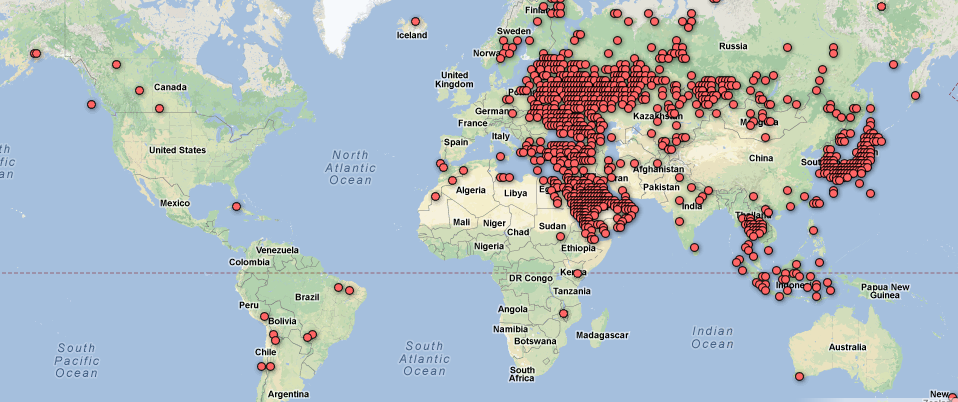
\includegraphics[scale=0.5]{unknown_plot.png}
\caption{\footnotesize Plot showing the areas where the relative frequency of unknown tweets were $> 0.6$. We can see a lot of dots on places where the 5 supported languages are not spoken. Eg, Japan, Korea, parts of Europe, Saudi Arabia etc.}
\label{fig:s4}
\end{figure*}

In order to achieve this, the surface of the earth was divided into $1^{\circ}$ by $1^{\circ}$ geo-desic cells (similar to what was done in Wing and Baldridge (2011)). The geo-located tweets in each cell were then labeled using the High-confidence Dictionary-based approach. This would give us the probability distribution of languages for a particular cell. In other words, we have the relative frequencies of each language's occurrence in a given cell. We are likely to get better models for a language in regions where the relative frequency of that language is very high. For our experiments, optimal results were obtained when this threshold was set to 0.6. A cell is called ``highly reliable'' for a language $L$ if the relative frequency of tweets from that cell which are labeled as $L$ is at least 0.6.

%Figure 3 plots the $1^{\circ}$ by $1^{\circ}$ cells which have a high relative frequency for tweets labeled as ``Unknown'' by the High-confidence Dictionary-based approach. We can see clearly that regions like Saudi Arabia, China, Japan Korea, Thailand and parts of Europe are the predominant areas from where the tweets are labeled ``Unknown''. Similar plots were obtained for other languages as well, and the plots showed that using tweets from regions having high relative frequency for a language were much clearer and helped in reducing the noise. (This was visually verified, based on the language and the regions plotted on the map. For example, the ``highly reliable'' regions for Spanish tweets had a lot of cells in Mexico, Spain and South American regions. However, if we plotted all tweets labeled Spanish, we got a plot which contained a lot of noise -- mostly because of some isolated tweets or wrongly-labeled tweets).

The character n-grams collected from these ``highly reliable'' regions were then used in the model to predict languages in tweets. The results are reported in Table 3. We can see clearly that collecting training data from only the relevant regions increases the accuracy of prediction slightly. As in the other methods, when combined with the blogger prior of the tweet authors, the accuracy improves greatly. This approach gives the best overall accuracy for language identification task.

\section {Discussion}
In this section, some observations that were made while running the experiments are discussed. First of all, it is clear from the results section that, if we have large amounts of data that might not be entirely correctly labeled, it is still enough to train a model that performs very well. The task of language identification cannot be simply solved by counting the number of valid words from a language and reporting the language with the most words. We could find a lot of tweets which were misspelt, but were correctly labeled by our approach. These tweets would not be correctly predicted by the simple dictionary approach. For example, a tweet that contained just the word ``incredile'' (note the missing `b') was labeled as English by our approach, but was labeled as Unknown by the dictionary based method. On manual inspection, we could find quite a few tweets (at least in English) that were misspelt.



\section{Conclusion}
In this paper, an unsupervised method for labeling tweets with language was described. It is a very conservative and simple approach which does not necessarily label all the tweets in the dataset. It works by labeling the tweets which contain enough number of valid words from a language, and also meets the criterion of the proportion of valid words in the tweet. When there are a large number of tweets available, a considerable amount of labeled data is obtained. We also show that, the labeled data obtained by this method is very reliable and performs on par with the existing methods for language detection. Thus, the tedious task of manually labeling the tweets with languages can be replaced with our unsupervised labeling algorithm which depends only on the dictionary of a language. It was also shown that an overall accuracy of around 92\% was achieved for the task of language detection. Results were shown for five languages -- English, Spanish, French, German and Dutch.

\begin{thebibliography}{}

\bibitem[\protect\citename{Carter et al}2012]{SC:2012}
Carter, S. and Weerkamp, W. and Tsagkias, E.
\newblock 2012.
\newblock Microblog Language Identification: Overcoming the Limitations of Short, Unedited and Idiomatic Text.
\newblock {\em Language Resources and Evaluation Journal}.

\bibitem[\protect\citename{Chen}2011]{SC:2011}
Chen, Edwin.
\newblock 2011.
\newblock Filtering for English Tweets: Unsupervised Language Detection on Twitter.
\newblock {\em http://blog.echen.me/2011/05/01/unsupervised-language-detection-algorithms}.

\bibitem[\protect\citename{Hong}2011]{HC:2011}
Hong, L., Convertino, G. and Chi, E.
\newblock 2011.
\newblock Language matters in twitter: A large scale study.
\newblock In {\em In International AAAI Conference on Weblogs and Social Media}.

\bibitem[\protect\citename{semiocast}2010]{se:2010}
Semiocast.
\newblock 2010.
\newblock Half of messages on twitter are not in english: japanese is the second most used language.
\newblock {\em http://semiocast.com/downloads/semiocast half\_of\_messages\_on\_twitter\_are\_not\_in\_english\_20100224.pdf}.


\bibitem[\protect\citename{Han}2011]{se:2011}
Han, Bo and Baldwin, Timothy.
\newblock 2011.
\newblock Lexical normalisation of short text messages: makn sens a \#twitter.
\newblock {\em Proceedings of the 49th Annual Meeting of the Association for Computational Linguistics: Human Language Technologies - Volume 1}.

\bibitem[\protect\citename{Tromp}2011]{TR:2011}
Tromp, Erik and Pechenizkiy, Mykola.
\newblock 2011.
\newblock Graph-Based N-gram Language Identification on Short Texts.
\newblock {\em Proceedings of the Twntieth Belgian Dutch Conference on Machine Learning Benelearn 2011}.

\bibitem[\protect\citename{Ceylan}2011]{CE:2011}
Ceylan, Hakan and Kim, Yookyung.
\newblock 2009.
\newblock Language identification of search engine queries.
\newblock {\em Proceedings of the Joint Conference of the 47th Annual Meeting of the ACL and the 4th International Joint Conference on Natural Language Processing of the AFNLP: Volume 2}.

\bibitem[\protect\citename{Carter2}2011]{CAR:2011}
Carter, Simon and Tsagkias, Manos and Weerkamp, Wouter
\newblock 2011.
\newblock Semi-Supervised Priors for Microblog Language Identification.
\newblock {\em Dutch-Belgian Information Retrieval workshop (DIR 2011)}.

\bibitem[\protect\citename{Bal}2010]{Bal:2010}
Baldwin, Timothy and Lui, Marco.
\newblock 2010.
\newblock Language identification: the long and the short of the matter.
\newblock {\em Human Language Technologies: The 2010 Annual Conference of the North American Chapter of the Association for Computational Linguistics}.

\bibitem[\protect\citename{Weerkamp}2011]{Wee:2011}
Weerkamp, W. and Carter, S. and Tsagkias, E.
\newblock 2011.
\newblock How People use Twitter in Different Languages.
\newblock {\em Web Science 2011}.

\bibitem[\protect\citename{Wing}2011]{Win:2011}
Wing, B. and Baldridge, J.
\newblock 2011.
\newblock  Simple supervised document geolocation with geodesic grids.
\newblock {\em Proceedings of ACL HLT 2011}.

\bibitem[\protect\citename{Nigam}2000]{Nigam:2000}
Nigam, K. and McCallum, A. and Thrun, S. and Mitchell, T.
\newblock 2000.
\newblock  Text Classification from Labeled and Unlabeled Documents using EM.
\newblock {\em Machine Learning}.


\end{thebibliography}

\end{document}
